\documentclass[12pt]{article}
\usepackage{setspace,graphicx,amsmath,geometry,fontspec,titlesec,soul,bm,subfigure}
\titleformat{\section}[block]{\LARGE\bfseries}{\arabic{section}}{1em}{}[]
\titleformat{\subsection}[block]{\Large\bfseries\mdseries}{\arabic{section}.\arabic{subsection}}{1em}{}[]
\titleformat{\subsubsection}[block]{\normalsize\bfseries}{\arabic{subsection}-\alph{subsubsection}}{1em}{}[]
\titleformat{\paragraph}[block]{\small\bfseries}{[\arabic{paragraph}]}{1em}{}[]
\setmainfont{Times New Roman}
\renewcommand{\baselinestretch}{1.15}
\geometry{a4paper,left=2.5cm,right=2.5cm,top=2.5cm,bottom=2.5cm}
\begin{document}
	\newpagestyle{main}{            
		\sethead{Ziqing Yu}{Bildverarbeitung 1}{3218051}     
		\setfoot{}{\thepage}{}
		\headrule
		\footrule
			}
	\pagestyle{main}

\section{Lineare Skalierung}
Die Maßstab und Offset(für alle Grauwerte). \newline
\begin{equation*}
k_{1}=\frac{255-0}{224-74}=1,7000\ \ \ \ \ \ \ \ \ b_{1}=\frac{224 \cdot 0-74 \cdot 255}{224-74}=-125,8000    
\end{equation*}
Die max. und min. Grauwerte sind 146 und 82, wenn jeweils $5\%$ der dunkelsten bzw. hellsten Grauwerten weg sind. Die Maßstab und Offset(ohne jeweils $5\%$ dunkelsten bzw. hellsten Grauwerten).
\begin{equation*}
k_{2}=\frac{255-0}{146-82}=3,9844\ \ \ \ \ \ \ \ \ b_{2}=\frac{146 \cdot 0-82 \cdot 255}{146-82}=-326,7188    
\end{equation*}
\begin{equation*}
I_{new}=k \cdot I_{old} + b
\end{equation*}
\begin{figure}[ht]\centering
	\subfigure[Originales Bild pout.tif]{
		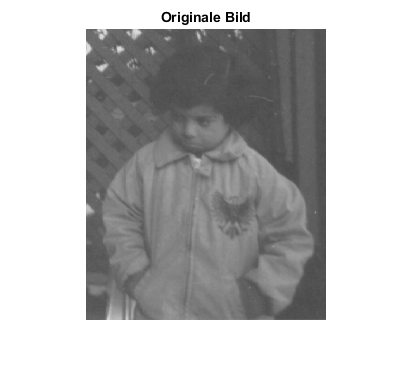
\includegraphics[width=0.3\textwidth]{originalbild.png}}
	\subfigure[Skaliertes Bild]{
		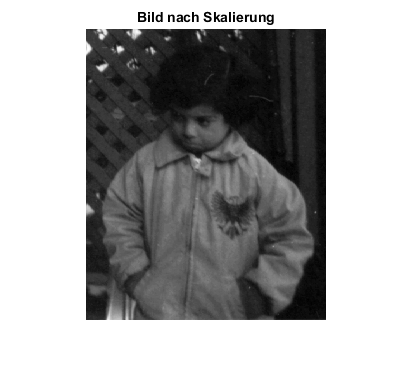
\includegraphics[width=0.3\textwidth]{BildSkalierung.png}}
	\subfigure[Skaliertes Bild(ohne 5\% jeweils dunkelste bzw. helleste Grauwerte)]{
		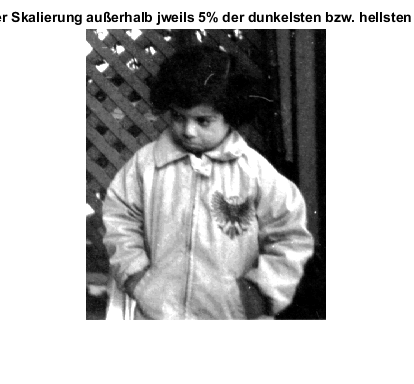
\includegraphics[width=0.3\textwidth]{BildSkalierung2.png}}
	\caption{Bilden}
\end{figure}
\begin{figure}[ht]\centering
	\subfigure[Histogramm des originalen Bildes]{
		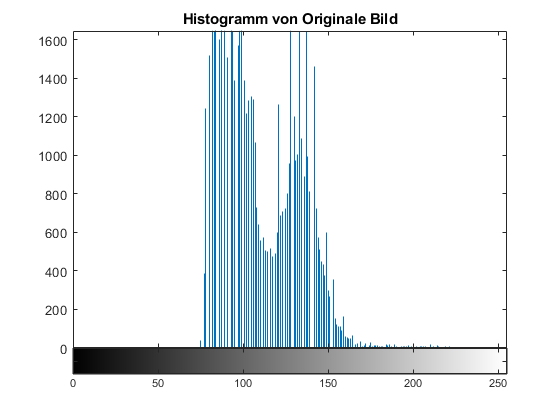
\includegraphics[width=0.3\textwidth]{HistogrammoriginalBild.png}}
	\subfigure[Histogramm des skalierte Bildes]{
		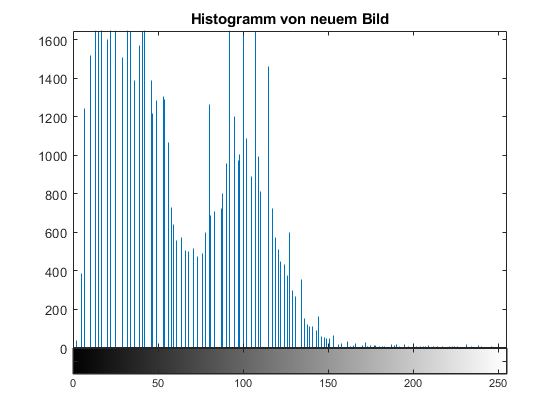
\includegraphics[width=0.3\textwidth]{HistogrammSkalierung.png}}
	\subfigure[Histogramm des skalierte Bild(ohne 5\% jeweils dunkelste bzw. helleste Grauwerte)]{
		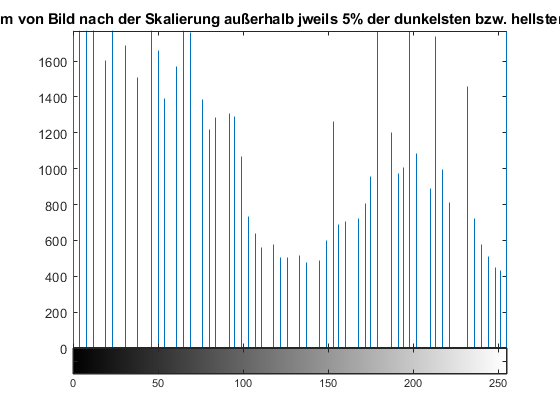
\includegraphics[width=0.3\textwidth]{HistogrammSkalierung2.png}}
	\caption{Histogramm}
\end{figure}

\section{Histogrammverebnung}
Das kummulative Histogramm wird als Transferfunktion zur Histogrammverebnung genutzt, weil das normierte Histogramm der Wahrscheinlichkeitverteilung entspricht und das reicht möglichst die Gleichverteilung der Grauwerte.
\begin{equation*}
I_{k}^{neu}=I_{max} \cdot \sum\limits_{j=0}^k \frac{n_j}{n}\ \ \ \ mit \ \  I_{max}=255
\end{equation*}
\begin{figure}[ht]\centering
	\subfigure[Originales Bild pout.tif]{
		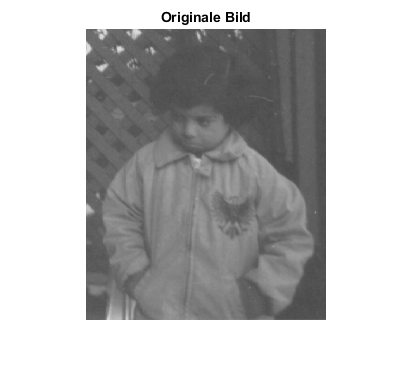
\includegraphics[width=0.45\textwidth]{originalbild.png}}
	\subfigure[Bild nach Verebnung]{
		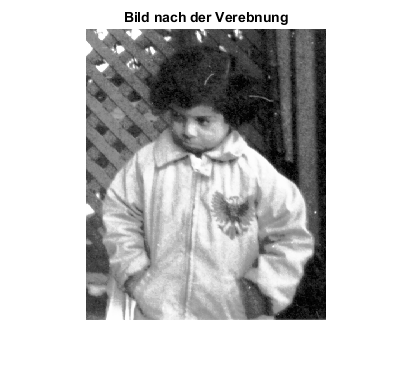
\includegraphics[width=0.45\textwidth]{BildVerebnung.png}}
	\caption{Bild Verebnung}
\end{figure}
\begin{figure}[ht]\centering
	\subfigure[Histogramm des originalen Bildes]{
		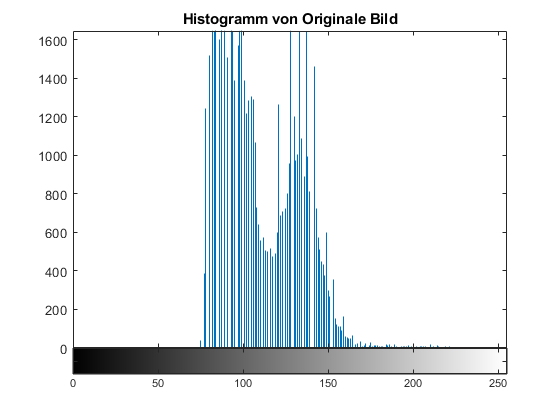
\includegraphics[width=0.45\textwidth]{HistogrammoriginalBild.png}}
	\subfigure[Histogramm des Bildes nach Verebnung]{
		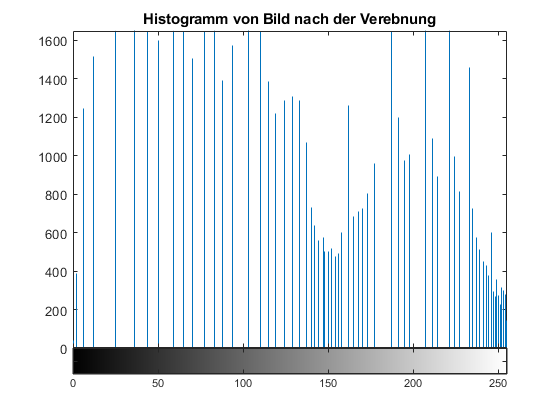
\includegraphics[width=0.45\textwidth]{HistogrammVerebnung.png}}
	\caption{Histogramm}
\end{figure}
\newpage
\section{Histogrammanpassung}
8874.jpg wird hier zu 8873.jpg angepassen. Zunächst werden beide kummulative Histogramme gerechnet. Dann mit diesen beiden Histogrammen kann man $I_{equal}$ durch die analoge Wahrscheinlichkeitsverteilung bestimmen, dann wird die Übertragungsfunktion gegriefen werden, danach ist die zuzuweisenden Grauwerte $I_2$ aus der Übertragungsfunktion bestimmen. 
\begin{figure}[ht]\centering
	\subfigure[8873.jpg]{
		\includegraphics[width=0.45\textwidth]{linkbild.png}}
	\subfigure[8874.jpg]{
		\includegraphics[width=0.45\textwidth]{rechtbild.png}}
	\caption{originale Bilden}
\end{figure}
\begin{figure}[ht]\centering
	\subfigure[8873.jpg]{
		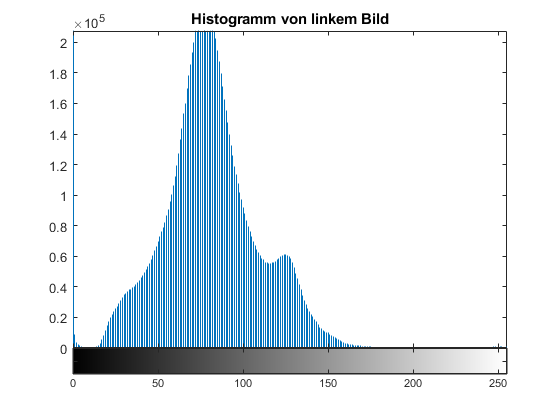
\includegraphics[width=0.45\textwidth]{Histogrammlink.png}}
	\subfigure[8874.jpg]{
		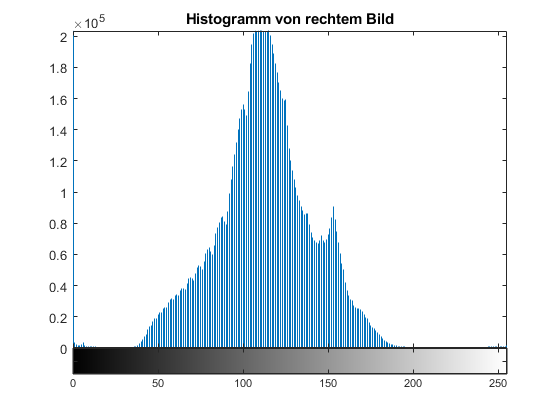
\includegraphics[width=0.45\textwidth]{Histogrammrecht.png}}
	\caption{Histogramm der originalen Bilden}
\end{figure}
\begin{figure}[ht]\centering
	\subfigure[8873.jpg]{
		\includegraphics[width=0.45\textwidth]{linkbild.png}}
	\subfigure[8874.jpg nach Anpassung zu 8873.jpg]{
		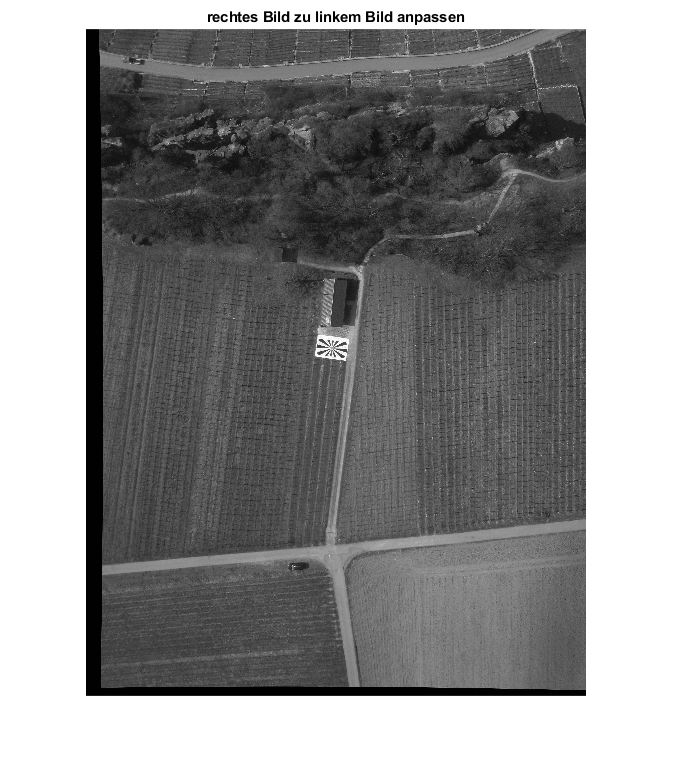
\includegraphics[width=0.45\textwidth]{RzuLanpassen.png}}
	\caption{Anpassung}
\end{figure}
\begin{figure}[ht]\centering
	\subfigure[Histogramm von 8873.jpg]{
		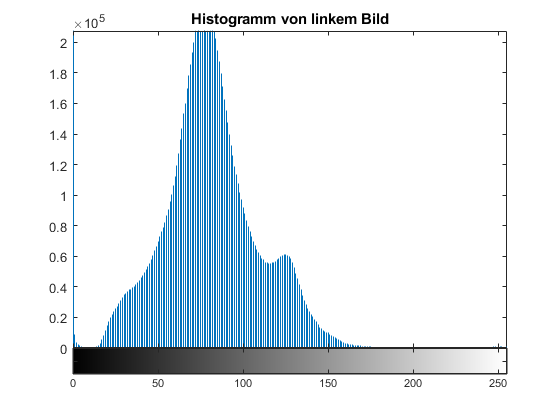
\includegraphics[width=0.3\textwidth]{Histogrammlink.png}}
	\subfigure[Histogramm von 8874.jpg nach der Anpassung]{
		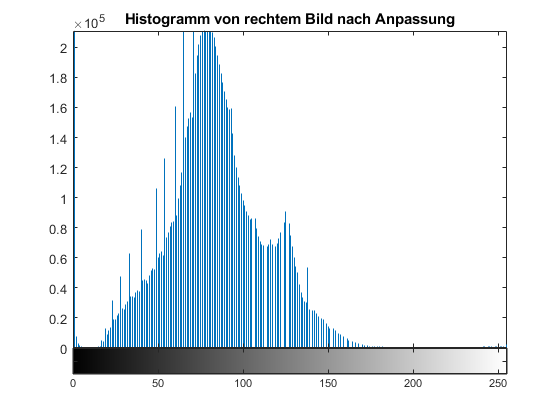
\includegraphics[width=0.3\textwidth]{Histogrammanpassung.png}}
	\subfigure[Histogramm von 8874.jpg nach der Anpassung (mit histeq)]{
		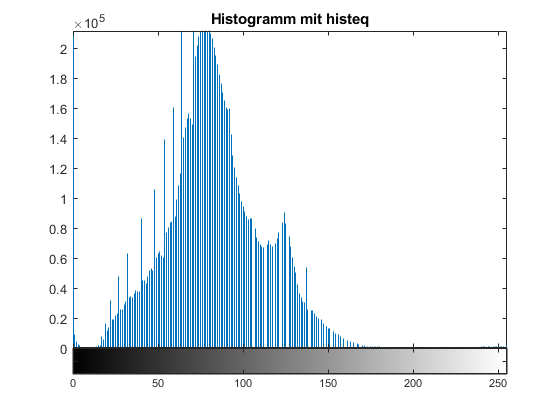
\includegraphics[width=0.3\textwidth]{histeq.png}}
	\caption{Histogramm nach Anpassung}
\end{figure}
\end{document}